%Struktur: 20 min Vortrag mit 1,5 min pro Folie -> 15 Folien inkl. Titelfolie
%10 min Fragen

%%%%%%%%%%%%%%%%%%%%%%%%%%%%%%%%%%%%%%%%%%%%%%%%%%%%%%%%%%%%%%%%%%%%%%%%%%%%%%%%%%%%%%%%%%%%%%%%%%%%%%%%%%%%%%%%%%%%%%%%%%%%%%%%%%%%%%

\documentclass[colorbacktitle,inverttitle,landscape,presentation,
	english,
	aspectratio=43, %43 or 169, 1610
	accentcolor=tud9b, %tud9b (temf) or tud5b (gsce) 
]{tudbeamer}

%%additional packages(Praesentation)
%%standard:

%%language:
\usepackage[utf8]{inputenc}
\usepackage[english]{babel}
%%math:
\usepackage{amsmath}
\usepackage{caption}
\usepackage{subcaption}
%%tikz:
\usepackage{tikz}
\usetikzlibrary{patterns}
\usepackage[siunitx,americaninductors]{circuitikz}
\usepackage{siunitx}
%%pgfplots:
\usepackage{pgfplots}
\usepgfplotslibrary{groupplots}
\usepgfplotslibrary{patchplots}
\usepackage{pgfplotstable}
\pgfplotsset{compat=newest}\usepgfplotslibrary{units}
%%scaling:
\usepackage{adjustbox}
\usepackage{wrapfig,lipsum,booktabs}
%%additional packages(Praesentation)
 

%needs to come last
\usepackage{temfbeamer}

%remove TU logo from every slide but the title
\setbeamertemplate{headline}[TUD theme nologo] 

%set date
\date{20. Juni, 2018}



%%%%%%%%%%%%%%%%%%%%%%%%%%%%%%%%%%%%%%%%%%%%%%%%%%%%%%%%%%%%%%%%%%%%%%%%%%%%%%%%%%%%%%%%%%%%%%%%%%%%%%%%%%%%%%%%%%%%%%%%%%%%%%%%%%%%%%

\title{Generierung des Eingangssingals für Barrier Bucket RF Systeme and der GSI }

\subtitle{\\[0.3\baselineskip]
	Jonas Christ, Artem Moskalew, Maximilian Nolte \\
{\small Jens Harzheim, M.Sc.}\\
[0.3\baselineskip]
{\tiny Projektseminar Beschleunigertechnik}\\[0.3em]
	\mbox{\scriptsize}~}
	
\institute[TU Darmstadt | Fachbereich 18 | Institut Theorie Elektromagnetischer Felder]{Institut für Theorie Elektromagnetischer Felder, TU Darmstadt}

%%%%%%%%%%%%%%%%%%%%%%%%%%%%%%%%%%%%%%%%%%%%%%%%%%%%%%%%%%%%%%%%%%%%%%%%%%%%%%%%%%%%%%%%%%%%%%%%%%%%%%%%%%%%%%%%%%%%%%%%%%%%%%%%%%%%%%

\begin{document}
	
\begin{titleframe}
	\tudtitle[images/temf_logo.pdf]{images/temf_background.jpg} 
	%\tudtitle[images/gsce_logo.pdf]{images/gsce_background.jpg}
	\end{titleframe}
	
\begin{frame}
	\frametitle{Outline}
	\tableofcontents%[currentsection,subsectionstyle=show/show/hide]
\end{frame}
	
%%%%%%%%%%%%%%%%%%%%%%%%%%%%%%%%%%%%%%%%%%%%%%%%%%%%%%%%%%%%%%%%%%%%%%%%%%%%%%%%%%%%%%%%%%%%%%%%%%%%%%%%%%%%%%%%%%%%%%%%%%%%%%%%%%%%%%

\section{Einführung}

\subsection{Problemstellung}
\begin{frame}{Problemstellung}

\begin{itemize}
	
	\item Barrier-Bucket System \uncover<2-> {: 
		\begin{itemize}
			\item Longitudinale Manipulation der Bunches
		\end{itemize}
		}
	\item Ziel \uncover<3-> {:
		\begin{itemize}
			\item Gap Spannung in Form einer Ein-Sinus Periode
			\item Qualität das Signals
		\end{itemize}
		}
		
		%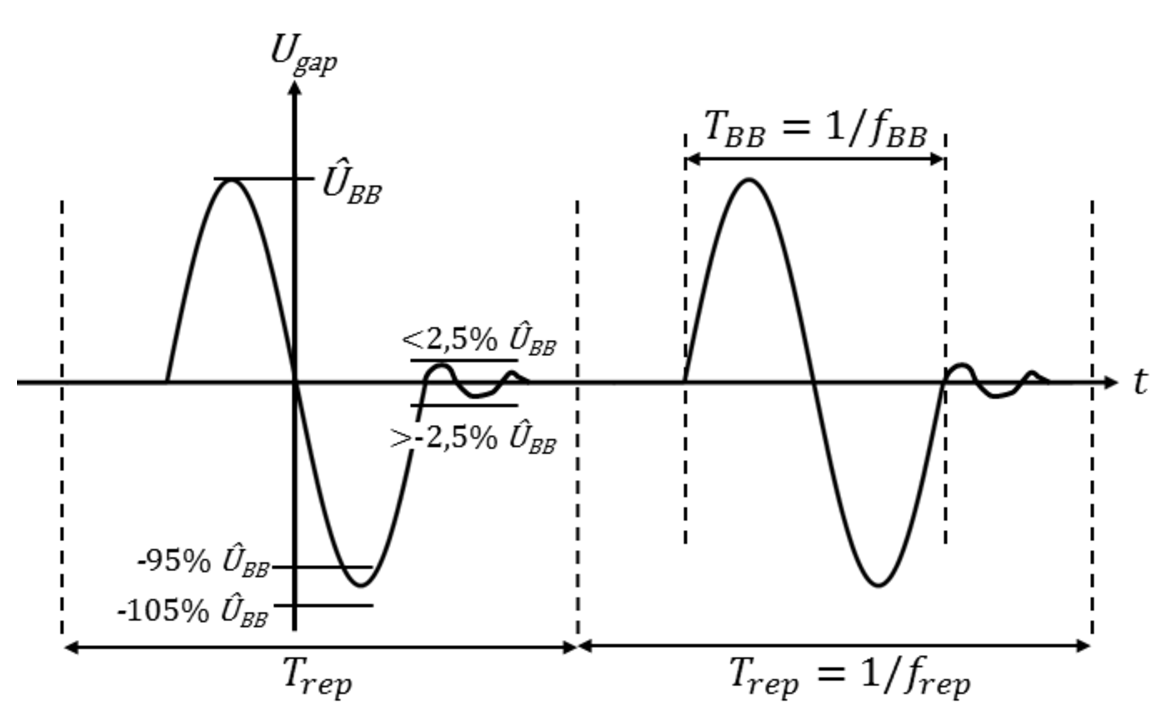
\includegraphics[scale=0.3]{slides/Problemstellung/BB_req.eps}
\end{itemize}		
\uncover<3-> {		
	\begin{picture}(10,7)
		\put(70,-90){
			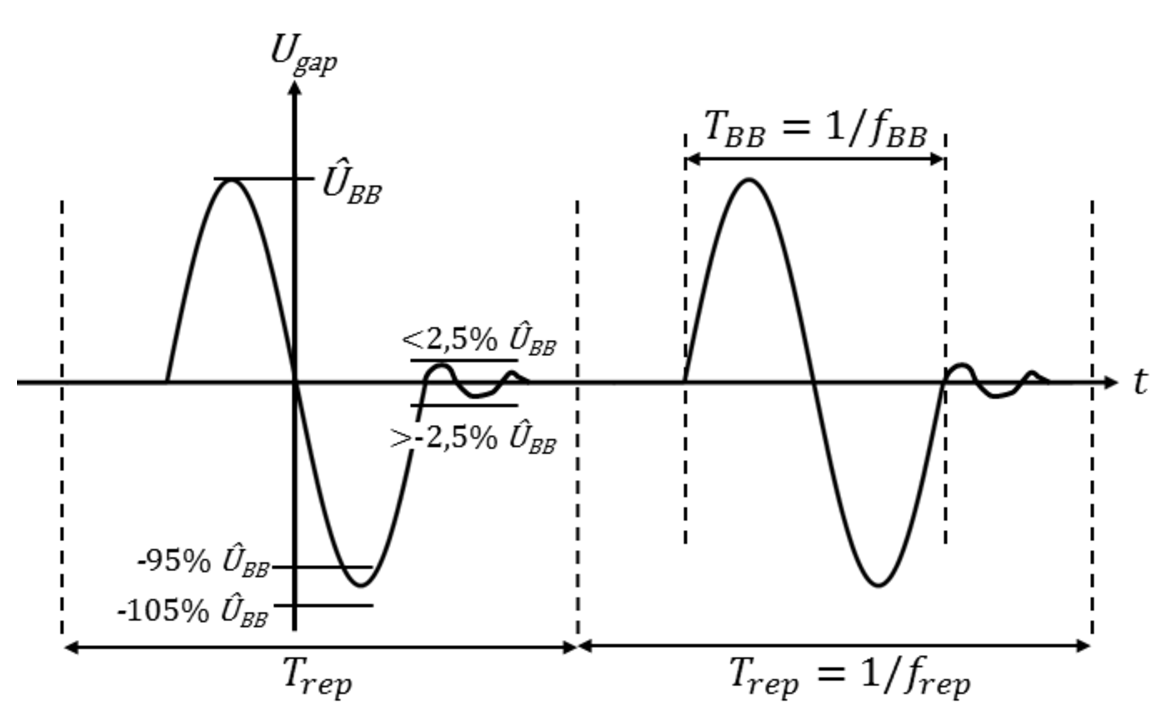
\includegraphics[scale=0.3]{slides/Problemstellung/BB_req.eps} 
		}  
	\end{picture} 
}	

\end{frame}





\subsection{Zielsetzung}
\begin{frame}{Zielsetzung}

\end{frame}





\subsection{Gegeben}
\begin{frame}{Gegeben}

\only<2->{ FFT.py \\[1\baselineskip] }
\only<1->{ MLBS.py \\[1\baselineskip] }
\only<3->{ getH.py \\[1\baselineskip] }
\only<4->{ computeUin.py \\[1\baselineskip] }
\only<5->{ runme\_compute.py \\[1\baselineskip] }

\end{frame}





\section{Erreichtes}

\subsection{Gerätekommunikation}
\begin{frame}{Erreichtes: das VISA-Handbuch}

\end{frame}





\subsection{Code}


\begin{frame}[fragile]
\ifnum\WertA=1
\frametitle{Code: Das Design}
\else
\frametitle{Code: Evaluierung}
\fi

%\only<1>
%	{ 
%\framebox{   %   % just so you can see where the "picture" is

\setcounter{onlyAt}{0}

\ifnum\WertA=1

\setcounter{onlyAt}{\value{onlyAt}+1}
\only<\value{onlyAt}>
{
	\begin{center}
		\includegraphics[scale=0.45]{slides/ResultCode/WEPVA047f2_2-eps-converted-to.pdf} 
	\end{center}
}

\setcounter{onlyAt}{\value{onlyAt}+1}
\only<\value{onlyAt}>
	{
	\begin{picture}(100,70)
		\put(15,0){
			\includegraphics[scale=1.0]{slides/ResultCode/Slide1.eps} 
		}  
	\end{picture} 
	}
\fi
		
\setcounter{onlyAt}{\value{onlyAt}+1}
\only<\value{onlyAt}>
	{
	\begin{picture}(100,70)
		\put(15,0){
			\includegraphics[scale=1.0]{slides/ResultCode/Slide2.eps} 
		}  
	\end{picture} 
	}
	


\ifnum\WertA=1 \setcounter{from}{\value{onlyAt}+1} \setcounter{till}{\value{onlyAt}+1} \else \setcounter{from}{\value{onlyAt}+1} \setcounter{till}{\value{onlyAt}+2} \fi	
\only<\value{from} - \value{till}> 
	{
	\begin{picture}(100,70)
		\put(15,0){
			\includegraphics[scale=1.0]{slides/ResultCode/Slide3.eps} 
		}  
	\end{picture} 
	\lstinputlisting[firstline=1,lastline=1]{slides/ResultCode/file.txt} 
	}	
	
\ifnum\WertA=2
	\setcounter{onlyAt}{\value{from} + 1}
	\only<\value{onlyAt}>
	{
		\begin{textblock}{20}(80,50)
    		\includegraphics[height=3.5cm, width=4.5cm ]{slides/ResultCode/plots/Uout_ideal.pdf} 
		\end{textblock}	
	} 	
\fi	
\setcounter{onlyAt}{\value{till}}


\ifnum\WertA=1 \setcounter{from}{\value{onlyAt}+1} \setcounter{till}{\value{onlyAt}+1} \else \setcounter{from}{\value{onlyAt}+1} \setcounter{till}{\value{onlyAt}+2} \fi	
\only<\value{from} - \value{till}> 
	{
	\begin{picture}(100,70)
		\put(15,0){
			\includegraphics[scale=1.0]{slides/ResultCode/Slide4.eps} 
		}  
	\end{picture} 
	\lstinputlisting[firstline=1,lastline=2]{slides/ResultCode/file.txt} 
	}
	
\ifnum\WertA=2
	\setcounter{onlyAt}{\value{from} + 1}
	\only<\value{onlyAt}>
	{
		\begin{textblock}{20}(93,50)
    		\includegraphics[ width=3.5cm, height=3.1cm ]{slides/ResultCode/plots/H_p.pdf} 
		\end{textblock}			
		\begin{textblock}{20}(61,50)
    		\includegraphics[ width=3.5cm, height=3.1cm]{slides/ResultCode/plots/H_a.pdf} 
		\end{textblock}	
		
	} 	 
\fi	
\setcounter{onlyAt}{\value{till}} 

\setcounter{onlyAt}{\value{onlyAt}+1}
\only<\value{onlyAt}>
	{
	\begin{picture}(100,70)
		\put(15,0){
			\includegraphics[scale=1.0]{slides/ResultCode/Slide5.eps} 
		}  
	\end{picture} 
	\lstinputlisting[firstline=1,lastline=3]{slides/ResultCode/file.txt} 
	}	
	
\setcounter{onlyAt}{\value{onlyAt}+1}
\only<\value{onlyAt}>
	{
	\begin{picture}(100,70)
		\put(15,0){
			\includegraphics[scale=1.0]{slides/ResultCode/Slide5-1.eps} 
		}  
	\end{picture} 
	\lstinputlisting[firstline=1,lastline=3]{slides/ResultCode/file.txt} 
	}
	
\ifnum\WertA=2
	\setcounter{from}{\value{onlyAt}} 
	\setcounter{till}{\value{onlyAt}+2}
	\only<\value{from} - \value{till}>
	{
		\begin{textblock}{20}(80,50)
    		\includegraphics[height=3.5cm, width=4.5cm ]{slides/ResultCode/plots/U_quest_ideal.pdf} 
		\end{textblock}	
	} 
\fi	

\setcounter{onlyAt}{\value{onlyAt}+1}
\only<\value{onlyAt}>
{
	\begin{picture}(100,70)
		\put(15,0)
		{
			\includegraphics[scale=1.0]{slides/ResultCode/Slide6.eps} 
		}  
	\end{picture} 
	\lstinputlisting[firstline=1,lastline=3]{slides/ResultCode/file.txt} 
}

\setcounter{onlyAt}{\value{onlyAt}+1}
\only<\value{onlyAt}>
{
	\begin{picture}(100,70)
		\put(15,0)
		{
			\includegraphics[scale=1.0]{slides/ResultCode/Slide7.eps} 
		}
	\end{picture} 	
	\lstinputlisting[firstline=1,lastline=4]{slides/ResultCode/file.txt} 	
}	

\setcounter{onlyAt}{\value{onlyAt}+1}
\only<\value{onlyAt}>
{
	\begin{picture}(100,70)
		\put(15,0)
		{
			\includegraphics[scale=1.0]{slides/ResultCode/Slide7.eps} 
		}
	\end{picture} 	
	\lstinputlisting[firstline=1,lastline=5]{slides/ResultCode/file.txt} 		

}

\ifnum\WertA=1 \setcounter{from}{\value{onlyAt}+1} \setcounter{till}{\value{onlyAt}+1} \else \setcounter{from}{\value{onlyAt}+1} \setcounter{till}{\value{onlyAt}+3} \fi	
\only<\value{from} - \value{till}> 
{
	\begin{picture}(100,70)
		\put(15,0)
		{
			\includegraphics[scale=1.0]{slides/ResultCode/Slide8.eps} 
		}
	\end{picture} 	
	\lstinputlisting[firstline=1,lastline=5]{slides/ResultCode/file.txt} 		

}

\ifnum\WertA=2
	\setcounter{onlyAt}{\value{from}+1}
	\only<\value{onlyAt}>
	{
		\begin{textblock}{20}(80,50)
    		\includegraphics[height=3.5cm, width=4.5cm ]{slides/ResultCode/plots/Uout_measured.pdf} 
		\end{textblock}	
	} 
	\setcounter{onlyAt}{\value{from}+2}
	\only<\value{onlyAt}>
	{
		\begin{textblock}{20}(80,50)
    		\includegraphics[height=3.5cm, width=4.5cm ]{slides/ResultCode/plots/Uout_measured_cut.pdf} 
		\end{textblock}	
	} 
\fi
\setcounter{onlyAt}{\value{till}} 
 
\ifnum\WertA=1 \setcounter{from}{\value{onlyAt}+1} \setcounter{till}{\value{onlyAt}+1} \else \setcounter{from}{\value{onlyAt}+1} \setcounter{till}{\value{onlyAt}+2} \fi	
\only<\value{from} - \value{till}> 
{
	\begin{picture}(100,70)
		\put(15,0)
		{
			\includegraphics[scale=1.0]{slides/ResultCode/Slide9.eps} 
		}  
	\end{picture} 
	\lstinputlisting[firstline=1,lastline=6]{slides/ResultCode/file.txt} 
}	

\ifnum\WertA=2
	\setcounter{onlyAt}{\value{from} + 1}
	\only<\value{onlyAt}>
	{
		\begin{textblock}{20}(80,50)
    		\includegraphics[height=3.5cm, width=4.5cm ]{slides/ResultCode/plots/U_quest_measured.pdf} 
		\end{textblock}	
	}
\fi
\setcounter{onlyAt}{\value{till}} 
	
\setcounter{onlyAt}{\value{onlyAt}+1}
\only<\value{onlyAt}>
{
	\begin{picture}(100,70)
		\put(15,0){
			\includegraphics[scale=1.0]{slides/ResultCode/Slide10.eps} 
		}  
	\end{picture} 
	\lstinputlisting[firstline=1,lastline=7]{slides/ResultCode/file.txt} 
}



\ifnum\WertA=1 \setcounter{from}{\value{onlyAt}+1} \setcounter{till}{\value{onlyAt}+1} \else \setcounter{from}{\value{onlyAt}+1} \setcounter{till}{\value{onlyAt}+2} \fi	
\only<\value{from} - \value{till}> 
{
	\begin{picture}(100,70)
		\put(15,0)
		{
			\includegraphics[scale=1.0]{slides/ResultCode/Slide11.eps} 
		}  
	\end{picture} 
	\lstinputlisting[firstline=1,lastline=8]{slides/ResultCode/file.txt} 
}

\ifnum\WertA=2
	\setcounter{onlyAt}{\value{from} + 1}
	\only<\value{onlyAt}>
	{
		\begin{textblock}{20}(80,50)
    		\includegraphics[height=3.5cm, width=4.5cm ]{slides/ResultCode/plots/K.pdf} 
		\end{textblock}	
	} 
\fi	
\setcounter{onlyAt}{\value{till}}	

\setcounter{onlyAt}{\value{onlyAt}+1}
\only<\value{onlyAt}>
{
	\begin{picture}(100,70)
		\put(15,0)
		{
			\includegraphics[scale=1.0]{slides/ResultCode/Slide12-0.eps} 
		}  
	\end{picture} 
	\lstinputlisting[firstline=1,lastline=8]{slides/ResultCode/file.txt} 
}
	
\setcounter{onlyAt}{\value{onlyAt}+1}
\only<\value{onlyAt}>
{
	\begin{picture}(100,70)
		\put(15,0)
		{
			\includegraphics[scale=1.0]{slides/ResultCode/Slide12-01.eps} 
		}  
	\end{picture} 
	\lstinputlisting[firstline=1,lastline=8]{slides/ResultCode/file.txt} 
}
	
\setcounter{onlyAt}{\value{onlyAt}+1}
\only<\value{onlyAt}>
{
	\begin{picture}(100,70)
		\put(15,0)
		{
			\includegraphics[scale=1.0]{slides/ResultCode/Slide12.eps} 
		}  
	\end{picture} 
	\lstinputlisting[firstline=1,lastline=9]{slides/ResultCode/file.txt} 
}
	
\setcounter{onlyAt}{\value{onlyAt}+1}
\only<\value{onlyAt}>
{
	\begin{picture}(100,70)
		\put(15,0)
		{
			\includegraphics[scale=1.0]{slides/ResultCode/Slide13-0.eps} 
		}  
	\end{picture} 
	\lstinputlisting[firstline=1,lastline=9]{slides/ResultCode/file.txt} 
}

\setcounter{onlyAt}{\value{onlyAt}+1}
\only<\value{onlyAt}>
{
	\begin{picture}(100,70)
		\put(15,0)
		{
			\includegraphics[scale=1.0]{slides/ResultCode/Slide13-01.eps} 
		}  
	\end{picture} 
	\lstinputlisting[firstline=1,lastline=10]{slides/ResultCode/file.txt} 
}
	
\setcounter{onlyAt}{\value{onlyAt}+1}
\only<\value{onlyAt}>
{
	\begin{picture}(100,70)
		\put(15,0)
		{
			\includegraphics[scale=1.0]{slides/ResultCode/Slide13.eps} 
		}  
	\end{picture} 
	\lstinputlisting[firstline=1,lastline=11]{slides/ResultCode/file.txt} 
}

  
%	\begin{figure}[t]
%	
%%	
%	\end{figure}	
	%}
%\only<2>{ \lstinputlisting[firstline=1,lastline=2]{slides/ResultCode/file.txt} }
%\only<3>{ \lstinputlisting[firstline=1,lastline=3]{slides/ResultCode/file.txt} }
%\only<4>{ \lstinputlisting[firstline=1,lastline=4]{slides/ResultCode/file.txt} }
%\only<5>{ \lstinputlisting[firstline=1,lastline=5]{slides/ResultCode/file.txt} }
%\only<6>{ \lstinputlisting[firstline=1,lastline=6]{slides/ResultCode/file.txt} }
%\only<7>{ \lstinputlisting[firstline=1,lastline=7]{slides/ResultCode/file.txt} }
%\only<8>{ \lstinputlisting[firstline=1,lastline=8]{slides/ResultCode/file.txt} }
%\only<9>{ \lstinputlisting[firstline=1,lastline=9]{slides/ResultCode/file.txt} }
%\only<10>{ \lstinputlisting[firstline=1,lastline=10]{slides/ResultCode/file.txt} }


\end{frame}





\section{Evaluierung}
\subsection{Gerätekommunikation}
\begin{frame}{Dokumentation und Gerätekommunikation - Evaluierung}

%Stand letzter Test
\begin{itemize}
\uncover<2->{
\item Unvollständige Dokumentation:
\begin{itemize}
	\item Parameter und Return-Variablen dokumentieren
\end{itemize}
}
\uncover<3->{
\item Getestete Teile der Gerätekommunikation:
\begin{itemize}
	\item VISA-Protokoll und PyVisa Package Installation 
	\item Kommunikation mit AWG von anderem Laptop aus über USB
\end{itemize}
}
\uncover<4->{
\item Ausstehende Teile der Gerätekommunikation:
\begin{itemize}
	\item Kommunikation mit Oszilloskop von anderem Laptop
	\item Laufzeit: Status-Abfrage der Geräte mit \texttt{BUSY?} oder \texttt{*WAI}
	\item Anpassung der Auflösung des DSO
\end{itemize}
}

\end{itemize}
\end{frame}





\subsection{Code}
\begin{frame}{Evaluierung: Python-Code für die nichtlinere Verzerrung}

\end{frame}





\section{Ausblick}
\documentclass[../Report.tex]{subfiles}


\begin{document}


\chapter{Ausblick}
\label{chap:ausb}
---- In diesem Kapitel wird auf offene Fragen / neue Probleme / Anstöße für weitere Arbeiten eingegangen. Dabei sollte es um eher inhaltliche Aspekte gehen (u. U. wenig to dos für Code-Design) gegebenenfalls darf hier bei vielem auf die Erfahrungen aus den vorigen Kapiteln verwiesen werden und damit einen Übersichts-Charakter haben (erleichtert nachfolgenden Projekten die Arbeit) --- 

\section{---- Optimierung ----}
\label{sec:ausb.opti}
--- in dieser section werden die offenen Fragen / Anregungen in Bezug auf den Optimierungs-algorithmus dargelegt, etwa: \\
- Iterations-Reihenfolge mit Messungen: abwechselnd K / H optimieren und dann messen oder zwischen zwei Messungen beide optimieren? Oder erst das eine mit mehreren Messungen optimieren und dann das andere ?
\\
- sinnhaftigkeit / Grenzen des genutzten Algorithmus (Idee Jens) erfragen?
\\
- Problem / Frage nach Phasen-Optimierung des H-Optimierers
\\
- Umgang mit Rauschen, Null-Durchgängen o. ä. im H-Optimierer
\\
- Möglichkeiten der Optimierung: Durchlaufen lassen mit direkter Anpassung an steigende Amplituden? 
\\
- (offene Punkte K-Optimierung?)

\section{--- Gerätekomm---}
\label{sec:ausb.geraete}
--- in dieser Section werden weitere Punkte der Geräte-Komm aufgegriffen, etwa - die (geringe) Auflösung des AWG im Kontext der Optimierung (ggf. in \ref{sec:ausb.opti} besser?) , die Einbindung des neuen Oszis oder die Idee der Klassen-Implementierung 
%TODO: prüfe Redundanz mit Abschnitt Gerätekommunikation! nur eine Einbindung, wo ist sie sinnvoller? 

%TODO: Überlegung ausführen, ob RF-Tools einbinden hier sinnvoller ist als in "Offenen Fragen" im Abschnitt Code-Design?






\end{document}
	
	
\end{document}